\section{compilers}
\subsection{what is a compiler}
Simply stated, a compiler is a program that can read a program in one language - the source language - and translate it into an equivalent program in another language - the target language[...]. \mcp{aho}{1}

\subsection{evolution of programming languages}
\mcp{aho}{13}

\subsection{requirements to optimizations}
\mcp{aho}{16}

\subsection{optimizing compilers}
Programmers using a low-level language have more control over a computation and can, in principle, produce more efficient code. Unfortunately , lower-level programs are harder to write and - worse still - less portable, more prone to errors, and harder to maintain. Optimizing compilers include techniques to improve the performance of generated code, thus offsetting the inefficiency introduced by high-level abstractions. \mcp{aho}{17}

\subsection{compiler phases}


\subsection{compiler front end}
\begin{figure}[!htbp]
	\centering
	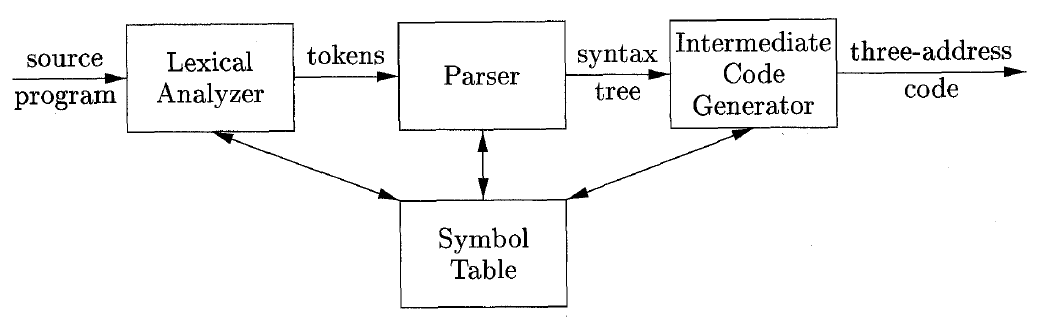
\includegraphics[width=1.0\linewidth]{PICs/compiler_front_end}
	\caption{Model of compiler front end \mcppic{aho}{41}.}\label{compiler_front_end}
\end{figure}

\subsection{AST}
In an \textit{abstract syntax tree} for an expression, each interior node represents an operator; the children of the node represent the operands of the operator. More generally, any programming construct can be handled by making up an operator for the construct and treating as operands the semantically meaningful components of that construct. \mcp{aho}{69}